\documentclass{beamer}
\beamertemplatenavigationsymbolsempty
\usecolortheme{beaver}
\setbeamertemplate{blocks}[rounded=true, shadow=true]
\setbeamertemplate{footline}[page number]
%
\usepackage[utf8]{inputenc}
\usepackage[demo]{graphicx}
\usepackage[english]{babel}
\usepackage{amssymb,amsfonts,amsmath,mathtext}
\usepackage{subfig}
\usepackage[all]{xy} % xy package for diagrams
\usepackage{natbib}
\usepackage{array}
\usepackage{comment}
\usepackage{multicol}% many columns in slide
\usepackage{hyperref}% urls
\usepackage{hhline}%tables
% Your figures are here:
\graphicspath{ {fig/} {../fig/} }

%----------------------------------------------------------------------------------------------------------
\begin{comment}
\title[\hbox to 56mm{Feature generation}]{Feature generation for classification and forecasting problems}
\author[N.\,P.~Ivkin]{Nikita Ivkin}
\institute{Moscow Institute of Physics and Technology}
\date{\footnotesize
\par\smallskip\emph{Course:} My first scientific paper\par (Strijov's practice)/Group 874 %821, 813
\par\smallskip\emph{Expert:} I.\,F.~Anny
\par\smallskip\emph{Consultant:} I.\,O.~Gordeos
\par\bigskip\small 2021}
\end{comment}

\title[]{Zero-order methods for Saddle Point}
\author{by Antyshev Tikhon}


\date[]{2022}

%---------------------------------------------------------------------------------------------------------
\begin{document}

\begin{frame}
\thispagestyle{empty}
\maketitle
\end{frame}

%----------------------------------------------------------------------------------------------------------
%----------------------------------------------------------------------------------------------------------
\begin{frame}{Establishing goals}
\begin{itemize}
    \item We consider following stochastic saddle point problem:
\begin{equation*}
    \min\limits_{x \in \mathcal{X}}\max\limits_{y \in \mathcal{Y}} f(x, y)
\end{equation*}
where $f(x, y) \stackrel{\mathsmaller{\mathsf{def}}}{=} \mathbb{E}_{\xi}f(x, y, \xi)$. 

\item However, we only possess zero-order oracle information. Derivatives either do not exist or are not available.

%\item Federated Learning avoids centralized data-storing and instead %relies on clients for greater energy efficiency and privacy.
\end{itemize}
%\begin{block}{Project goal}
%The goal of the project is solving the problem using Local SGD and %compare it to the Federated Random Reshuffling.
%\end{block}

\end{frame}
%-----------------------------------------------------------------------------------------------------
\begin{frame}{Gradient Approximation}
    \begin{itemize} 
        \item We assume that we can call a noise-corrupted zeroth-order oracle: $\phi(x,y,\xi)\stackrel{\mathsmaller{\mathsf{def}}}{=} f(x, y, \xi) + \delta(x,y)$

        \item To approximate gradient we pick two vectors from Euclidian sphere:$ \mathbf{e}_x, \mathbf{e}_y$ and define $\mathbf{e}= \begin{pmatrix}
            \mathbf{e}_x \\
            -\mathbf{e}_y
        \end{pmatrix}$

        \[g(x, y, \mathbf{e}) = \frac{d_x + d_y}{2\tau}\left(\phi\left((x,y) +\tau\mathbf{e}; \xi\right) - \phi\left((x,y) - \tau\mathbf{e}; \xi\right) \right)\cdot \mathbf{e}\]
    \end{itemize}
    
\end{frame}
%-----------------------------------------------------------------------------------------------------
\begin{frame}{Support Vector Machine SP}

\begin{itemize}
\item The Lagrangian of the SVM is:
\[\mathcal{L}(w, \lambda) = \frac{1}{2}\lVert w \rVert^2 + \sum\limits_{i=1}^l \lambda_i (1 - M_i(w))\]

\item This results in a SP:
\[ \min\limits_{w}\max\limits_{\lambda}\mathcal{L}(w, \lambda)\]

\end{itemize}
    
\end{frame}

\begin{frame}{Mirror Descent algorithm}
\begin{itemize}
    \item To solve the optimization task we will be using a zeroth-order modification of the Mirror Descent:
    \end{itemize}
    \bigskip
    \begin{figure}
        \centering
        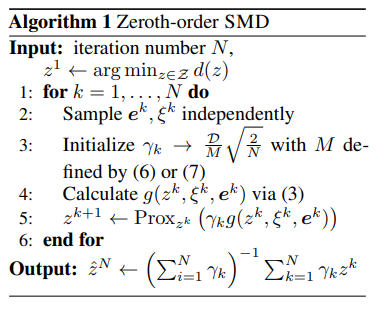
\includegraphics[scale=0.4]{alg_smd.png}
        \caption{The 0-order MD algorithm}
        \label{fig:my_label}
    \end{figure}
    
\end{frame}

%----------------------------------------------------------------------------------------------------------
\begin{frame}{The Experiment}
\begin{itemize}
    \item The test is performed on a synthetic low-dimensional data.
\end{itemize}  

\begin{figure}
\centering
\begin{minipage}{.5\textwidth}
  \centering
  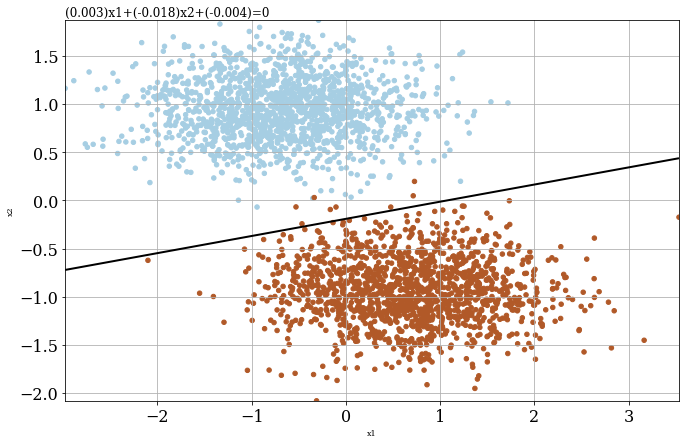
\includegraphics[width=.9\linewidth]{results2dim.png}
  \captionof{figure}{Visualized results}
  \label{fig:test1}
\end{minipage}%
\begin{minipage}{.5\textwidth}
  \centering
  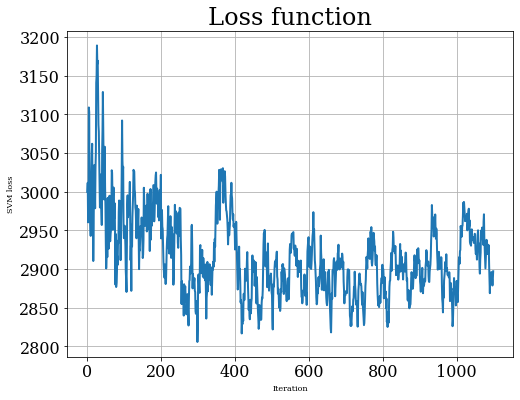
\includegraphics[width=.9\linewidth]{loss2dim.png}
  \captionof{figure}{Loss}
  \label{fig:test2}
\end{minipage}
\end{figure}




\end{frame}


%----------------------------------------------------------------------------------------------------------

\begin{frame}{Conclusion}

\begin{itemize}

    \item As a result we demonstrated, that zeroth order methods are capable of solving ML SP tasks.
    \item There are still more testing to be done in comparing Mirror Descent to Mirror Prox algorithm.
    
    \item It should also be tried on large classification task.
\end{itemize}
\end{frame}

%----------------------------------------------------------------------------------------------------------

\begin{frame}{References}
\nocite{*}
{\small
\bibliographystyle{unsrtnat}
\bibliography{references.bib}
}
\end{frame}
%----------------------------------------------------------------------------------------------------------
\begin{comment}

\begin{frame}{Solution}

\begin{columns}[c]
\column{0.6\textwidth}
    Column 1
\column{0.4\textwidth}
    Column 2
\end{columns}
\end{frame}

\end{comment}

%----------------------------------------------------------------------------------------------------------
\begin{comment}
\begin{frame}{Conclusion}
    \begin{block}{Forecast with hierarchical aggregation of}
    \begin{itemize}
        \item types of freight in
        \item stations, regions, and roads,
        \item for a day, week, month, and quarter.
    \end{itemize}
    \end{block}
\end{frame}
\end{comment}
%----------------------------------------------------------------------------------------------------------
\end{document} 
